%% START INTRO CHAPTER
\addcontentsline{toc}{chapter}{\introtitle}
\chapter*{\introtitle}
\newpage

Although they are typically associated with the study of the evolution of species, phylogenetic trees can be used to study the evolution of any sequence that evolves. For example, phylogenetic methods have been used to study the evolution of multicopy gene families~ \cite{Page1997}, cancer genomes~\cite{El-Kebir2016,Nowell1976}, antibodies~\cite{Litman1993,Robinson2015,Safonova2015}, segmental duplicates~\cite{Bailey2006,Jiang2007}, and transposable genomic elements~\cite{Dewannieux2003,Moshiri2017}, which are all entities that evolve \textit{within} the genome of a single species.

Models of tree evolution describe probability distributions over the space of tree shapes~\cite{Yule1925,Aldous2001}, which can be used as the prior distribution in a Bayesian inference~\cite{Drummond2007,Mooers2012,Sayyari2016}, to generate null distributions describing certain neutral processes~\cite{Guyer1991,Kirkpatrick1993,Agapow2002}, or to infer evolutionary parameters inherently of interest to the biologist~\cite{Morlon2014}. Similarly, generalized epidemic models describe probability distributions over the space of transmission networks~\cite{Sahneh2013}, and simulations that sample the distributions defined by these stochastic models allows epidemiologists to study infection patterns of disease epidemics~\cite{Sahneh2017}.

The spread of many infectious diseases is driven by social and sexual networks~\cite{Rivas2012}, and reconstruction of their transmission histories from molecular data can greatly enhance intervention. For example, network-based statistics for measuring \gls{hiv} treatment effects can yield increased statistical power~\cite{Wertheim2011}; the analysis of the growth of \gls{hiv} infection clusters can yield actionable epidemiological information for disease treatment and prevention~\cite{Aldous2012,Brenner2013}; transmission-aware models can be used to infer rates of \gls{hiv} evolution~\cite{Vrancken2014}. Multiple methods exist that utilize phylogenetic inference in the reconstruction of transmission networks~\cite{Prosperi2011,Ragonnet-Cronin2013,Moshiri2018b,Balaban2019}, but the accuracies, errors, and limitations of these methods are still poorly understood.

By utilizing models of viral transmission, tree evolution, and sequence evolution together, epidemiologists can simulate realistic data representative of a virus of interest as it spreads through a population of interest, and the resulting data can be used to evaluate the accuracies of transmission network inference methods as well as to study trends and patterns of an epidemic as a function of the various model parameters to gain insights into the mechanisms driving the epidemic of interest~\cite{Ratmann2017}.

%%% SAMPLE FIGURE
\begin{figure}[h] 
  \centering
  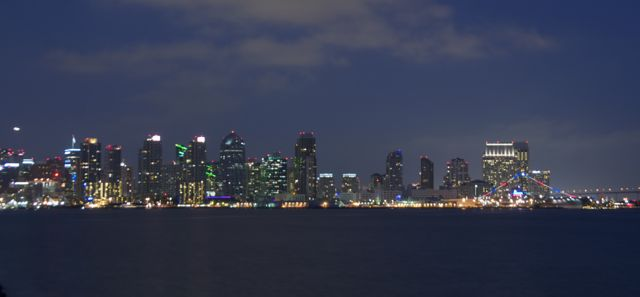
\includegraphics[width=0.5\textwidth]{sandiego}
  \caption[A picture of San Diego. Short figure caption must be \protect{$< 4$} lines in the list of figures]
{A picture of San Diego.  Short figure caption must be \protect{$< 4$} lines in the list of figures and match the start of the main figure caption verbatim. Note that figures must be on their own line (no neighboring text) and captions must be single-spaced and appear \protect\textit{below} the figure.  Captions can be as long as you want, but if they are longer than 4 lines in the list of figures, you must provide a short figure caption.\index{SanDiego}}
  \label{fig:sandiego}
\end{figure}

%%% SAMPLE TABLE
\vspace{0.25in}
\begin{table}[!ht]
\caption[A table of when I get hungry.  Short table caption must be \protect{$< 4$} lines in the list of tables]{A table of when I get hungry. Short table caption must be \protect{$< 4$} lines in the list of tables and match the start of the main table caption verbatim.  Note that tables must be on their own line (no neighboring text) and captions must be single-spaced and appear \protect\textit{above} the table.  Captions can be as long as you want, but if they are longer than 4 lines in the list of figures, you must provide a short figure caption.}
\vspace{-0.25in}
\begin{center}
\begin{tabular}{|p{1in}|p{2in}|p{3in}|}
\hline
Time of day & Hunger Level & Preferred Food \\
\hline
8am & high & IHOP (French Toast) \\
\hline
noon & medium & Croutons (Tomato Basil Soup \& Granny Smith Chicken Salad) \\
\hline
5pm & high & Bombay Coast (Saag Paneer) or Hi Thai (Pad See Ew) \\
\hline
8pm & medium & Yogurt World (froyo!) \\
\hline
\end{tabular}
\end{center}
\label{tab:analysis3}
\end{table}

%% END INTRO CHAPTER